In this chapter, the application of this thesis will be presented, with the above analysis applied to a swarm of UAVs. In addition, a variety of  simulations with different cost functions have been conducted to observe the motion of the agents, while ensuring boundedness and square integration of the proposed variables, in order to achieve optimal consensus. The simulations have been developed in MATLAB.

\section{Application}
    
    Consider a group of $N$ UAVs which are shown in figure \ref{fig:5.1}. From \cite{9213862} the kinematics of a UAV $i \in \mathcal{V}$  in 3-dimentional space are described by
    \begin{equation}\label{eq:5.1.1}
        \begin{align*}
            \dot{x}_i &= \hspace{2.0mm} V_i cos(\chi_i) cos(\gamma_i)\\
            \dot{y}_i &= \hspace{2.0mm} V_i sin(\chi_i) cos(\gamma_i)\\
            \dot{z}_i &= \hspace{2.0mm} V_i sin(\gamma_i)
        \end{align*}
    \end{equation}
    where $(x_i, y_i, z_i)$ denotes the position in the inertia frame, $V_i$ the speed of the UAV, $\chi_i$ the heading angle of the UAV and $\gamma_i$ the flight path angle of the UAV. The dynamics of the $i-$th UAV are described by
    \begin{equation}\label{eq:5.1.2}
        \begin{align*}
                \dot{V}_i &= \hspace{2.0mm}(T_i - D_i)/m_i - g sin(\gamma_i)\\
                \dot{\chi}_i &= \hspace{2.0mm}(L_i sin(\phi_i))/(m_i V_i cos(\gamma_i))\\
                \dot{\gamma_i} &= \hspace{2.0mm}(L_i cos(\phi_i) - m_i g cos(\gamma_i))/m_i V_i
        \end{align*}
    \end{equation}
    where $T_i$ is the engine thrust, $L_i$ the vehicle lift, $D_i$ the vehicle drag, $m_i$ the mass, $g$ the gravitational constant and $\phi_i$ the banking angle.
    \begin{figure}[H]
        \centering
        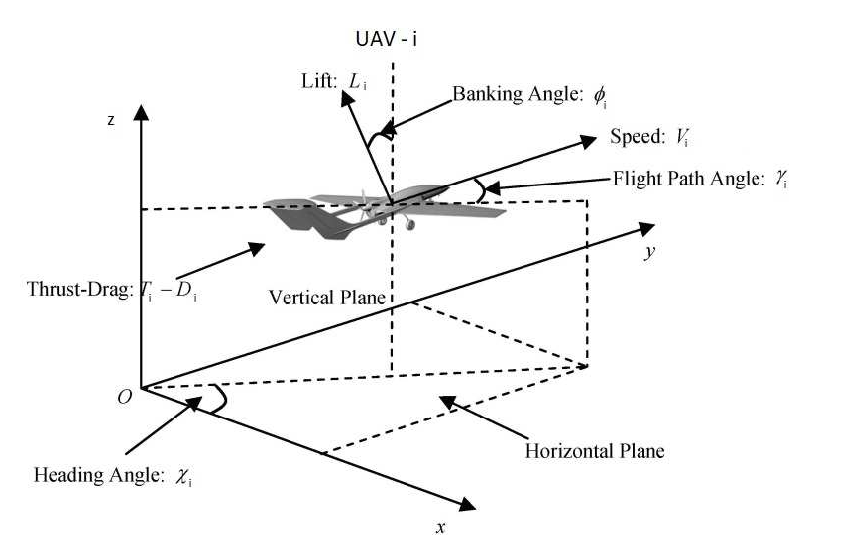
\includegraphics[width=0.8\linewidth]{images/Chapter5/UAV.png}
        \caption{Parameters of $i-$th UAV, \cite{9213862}.}
        \label{fig:5.1}
    \end{figure}
     Let $F_i = [T_i\hspace{3.0mm} L_isin(\phi_i)\hspace{5.0mm}  L_icos(\phi_i)]^T$ be the control input, $p_i = [x_i\hspace{5.0mm}  y_i\hspace{5.0mm}  z_i]^T$ the position vector and $v_i = \dot{p}_i = [\dot{x}_i\hspace{5.0mm}  \dot{y}_i\hspace{5.0mm}  \dot{z}_i]^T$ the velocity vector. Then, from the equations (\ref{eq:5.1.1}), (\ref{eq:5.1.2}) it is derived that
     \begin{equation}\label{eq:5.1.3}
         \begin{align*}
             \dot{p}_i &= \hspace{2.0mm} v_i\\
             m_i \dot{v}_i &= \hspace{2.0mm} \eta_i + m_i \varepsilon_i + G_iF_i
         \end{align*}
     \end{equation}
     where
     \begin{equation}\label{eq:5.1.4}
         \eta_i = \left[\begin{matrix}
             -D_i cos(\chi_i) cos(\gamma_i)\\
             -D_i sin(\chi_i) cos(\gamma_i)\\
             -D_i sin(\gamma_i)
         \end{matrix}\right]
     \end{equation}
     \vspace{2.0mm}
     \begin{equation}\label{eq:5.1.5}
         \varepsilon_i = [0 \hspace{2.0mm} 0 \hspace{2.0mm} g]^T
     \end{equation}
    and
    \begin{equation}\label{eq:5.1.6}
        G_i = \left[\begin{matrix}
            cos(\chi_i) cos(\gamma_i) & -sin(\chi_i) & -sin(\gamma_i) cos(\chi_i)\\
            sin(\chi_i) cos(\gamma_i) & cos(\chi_i) & -sin(\chi_i) cos(\gamma_i)\\
            sin(\gamma_i) & 0 & cos(\gamma_i)
        \end{matrix}\right]
    \end{equation}
    
    \vspace{4.0mm}
    
    It can be seen that $G_i^{-1} = G_i^T$. Every UAV communicate its position through the graph configuration in sampled time periods. Thus, its output is going to be $\boldsymbol{x}_i := \boldsymbol{p}_i$. Every UAV has a local nonconvex cost function $f_i(x_i,y_i,z_i)$ which is unknown. The algorithm \ref{alg:reg-prox-gpda} has a gradient approximation, thus only the information of the gradient is required in order to update the primal and dual variable. Consider that the input of the system is given by $F_i = G_i^T (u_i + d_i)$, with $u_i = [u_{i_x} \hspace{3.0mm} u_{i_y} \hspace{3.0mm} u_{i_z}]^T$ and $d_i = [d_{i_x} \hspace{3.0mm} d_{i_y} \hspace{3.0mm} 0]^T$. Then, the dynamics of every agent will be
    \begin{equation}\label{eq:5.1.7}
        \begin{align*}
             \dot{p}_i &= \hspace{2.0mm} v_i\\
             m_i \dot{v}_i &= \hspace{2.0mm} \eta_i + m_i \varepsilon_i + u_i + d_i\\
             x_i &= \hspace{2.0mm} p_i
         \end{align*}
    \end{equation}
     
\section{System Simulation with MATLAB}

    In this section, the simulations of the proposed algorithm with control scheme will be presented. The system is a network of $N = 5$ UAV agents which have dynamics from (\ref{eq:5.1.7}), and control laws of (\ref{eq:4.2.9}),(\ref{eq:4.2.10}). All the signals of the closed-loop system ought to be bounded, and the error variable tends to zero, as the agents reach the optimal stationary point.
    
\subsection{Parameters of the System}

    Every agent has a local cost function $f_i(x_i,y_i,z_i)$, $i\in \mathcal{V}$. The communication graph of the agents is shown in figure \ref{fig:5.2} . It can be seen that is connected as is perquisite of the assumption A.\ref{asm:4}.

    \begin{figure}[H]
        \centering
        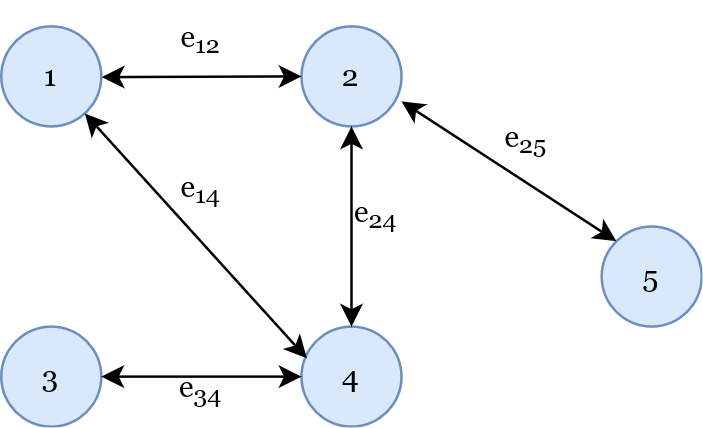
\includegraphics[width=0.5\linewidth]{images/Chapter5/Graph 1.png}
        \caption{Communication Graph of UAVs.}
        \label{fig:5.2}
    \end{figure}
    The incidence matrix of the communication graph of figure \ref{fig:5.2}, based on definition \ref{def:2.9} with its elements computed by equation (\ref{eq:2.1.1}), is
    \begin{equation*}
        \mathcal{A} = \left[\begin{matrix}
            1 & -1 & 0 & 0 & 0\\
            1 & 0 & 0 & -1 & 0\\
            0 & 1 & 0 & -1 & 0\\
            0 & 1 & 0 & 0 & -1\\
            0 & 0 & 1 & -1 & 0
        \end{matrix}\right]
    \end{equation*}

    The Laplacian matrix of the graph will be computed by equation (\ref{eq:2.1.3}), which is also the signed Laplacian. So
    \begin{equation*}
        L = L_- = \mathcal{A}^T\mathcal{A} =\left[\begin{matrix}
            1 & 1 & 0 & 0 & 0\\
            -1 & 0 & 1 & 1 & 0\\
            0 & 0 & 0 & 0 & 1\\
            0 & -1 & -1 & 0 & -1\\
            0 & 0 & 0 & -1 & 0
        \end{matrix}\right] \left[\begin{matrix}
            1 & -1 & 0 & 0 & 0\\
            1 & 0 & 0 & -1 & 0\\
            0 & 1 & 0 & -1 & 0\\
            0 & 1 & 0 & 0 & -1\\
            0 & 0 & 1 & -1 & 0
        \end{matrix}\right] = \left[ \begin{matrix}
            2 & -1 & 0 & -1 & 0\\
            -1 & 3 & 0 & -1 & -1\\
            0 & 0 & 1 & -1 & 0\\
            -1 & -1 & -1 & 3 & 0\\
            0 & -1 & 0 & 0 & 1
        \end{matrix}\right]
    \end{equation*}
    \begin{equation*}
        \Rightarrow L = \left[ \begin{matrix}
            2 & -1 & 0 & -1 & 0\\
            -1 & 3 & 0 & -1 & -1\\
            0 & 0 & 1 & -1 & 0\\
            -1 & -1 & -1 & 3 & 0\\
            0 & -1 & 0 & 0 & 1
        \end{matrix}\right]
    \end{equation*}
    The degree matrix of the graph can be computed from definitions (\ref{def:2.7}) and (\ref{def:2.8}). So,
    \begin{equation*}
        D = diag\{2,3,1,3,1\}
    \end{equation*}
    Finally, the signless Laplacian matrix will be computed from equation (\ref{eq:2.1.4}). So,
    \begin{equation*}
        L_{+} = 2D - \mathcal{A}^T\mathcal{A} = \left[\begin{matrix}
            4 & 0 & 0 & 0 & 0\\
            0 & 6 & 0 & 0 & 0\\
            0 & 0 & 2 & 0 & 0\\
            0 & 0 & 0 & 6 & 0\\
            0 & 0 & 0 & 0 & 2
        \end{matrix}\right] - \left[\begin{matrix}
            2 & -1 & 0 & -1 & 0\\
            -1 & 3 & 0 & -1 & -1\\
            0 & 0 & 1 & -1 & 0\\
            -1 & -1 & -1 & 3 & 0\\
            0 & -1 & 0 & 0 & 1
        \end{matrix}\right] = \left[\begin{matrix}
            2 & 1 & 0 & 1 & 0\\
            1 & 3 & 0 & 1 & 1\\
            0 & 0 & 1 & 1 & 0\\
            1 & 1 & 1 & 3 & 0\\
            0 & 1 & 0 & 0 & 1
        \end{matrix}\right]
    \end{equation*}

    The initial conditions of every $i-$th agent is presented by in the below vectors.
    \begin{equation*}
        \begin{align}
            x(0) &= [1, \hspace{3.0mm} 1.5, \hspace{3.0mm} 4, \hspace{3.0mm} -0.1, \hspace{3.0mm} 3]^T\\
            y(0) &= [0, \hspace{3.0mm} -2, \hspace{3.0mm} 1, \hspace{3.0mm} 5, \hspace{3.0mm} 2.5]^T\\
            z(0) &= [1, \hspace{3.0mm} 2.4, \hspace{3.0mm} 2, \hspace{3.0mm} 0.5, \hspace{3.0mm} 3.4]^T
        \end{align}
    \end{equation*}
    while the masses of the agents are presented in table \ref{tab:5.1}.
    \begin{table}[h]
        \centering
        \begin{tabular}{c c c c c c}
        \hline
            $i$ &  1 & 2 & 3 & 4 & 5\\
            $m_i (kg)$ & 2.1 & 3.2 & 2 & 1.8 & 2.8\\
        \hline
        \end{tabular}
        \caption{Mass of every agent.}
        \label{tab:5.1}
    \end{table}

    The parameters of the system that change in every scenario are presented in table \ref{tab:5.2}.
    \begin{table}[h]
        \centering
        \begin{tabular}{|c||c|}
        \hline
             Parameters &  Description\\
             \hline\hline
             $x_i(0)$,$y_i(0)$,$z_i(0)$ & Initial conditions of every agent\\
             \hline
             $x_{obs}$ & Position of an obstacle\\
             \hline
             $\tau$ & Obstacle distance\\
             \hline
             $S$, $U$ & Cost function constants\\
             \hline
             $D$ & Number of Delay Periods\\
             \hline
             $T$ & Sampled Period Time\\
             \hline
             $d_{max}$ & Communication delay\\
             \hline
             $\beta$ & penalty parameter\\
             \hline
             $c$ & Algorithm candidate function constant\\
             \hline
             $\epsilon$ & Algorithm convergence value\\
             \hline
             $\mathrm{L}$ & Lipschitz constant\\
             \hline
             $\vartheta_i$ & Sliding manifold gain parameters\\
             \hline
             $k_{i_1}$ & Controller gain\\
             \hline
             $\lambda_1$, $\lambda_2$ & Exponential gain parameters\\
        \hline
        \end{tabular}
        \caption{Variables of simulation}
        \label{tab:5.2}
    \end{table}



\subsection{Scenario 1: Optimal Consensus}
    As a first scenario of simulation, the local cost function will have a simple nonconvex form with $f_i(x_i) = \frac{1}{1 + e^{-a_ix_i}}$, with $a_i = \{2.4, 1.3, 0.5, 0.84, 1.25\}$.

















\subsection{Scenario 2: Optimal Consensus with Obstacle Avoidance}

    In the second scenario, the local cost function of every agent will have a different form to avoid a static obstacle. A good nonconvex suitable function for every agent is $f_i(x_i) =  \left \lVert x_i - x_i(0) \right \rVert^2 - \frac{\tau}{\tau + 1}  \left \lVert x_i - x_{obs} \right \rVert^2 $, with $\tau > 0$. With this cost function, the agents will achieve optimal consensus while avoiding a static obstacle with coordinates $x_{obs}$ and maintaining a short distance from the initial point $x_i(0)$ of every agent for reduced energy consumption, \cite{10125000}. The parameter $\tau$ sets the distance of the static obstacle from the agents. If $\tau = 0$ then the obstacle does not exist, while for an enormous value the obstacle has a significant distance from the agents' positions. In this, particular scenario is assumed that the distance parameter has value $\tau = 0.4$ and the coordinates of the obstacle are $x_{obs} = [1.5, \hspace{2.0mm} 2, \hspace{2.0mm} 1.8]^T$. 


















    
\subsection{Scenario 3: Formation Control with Obstacle Avoidance}

    Apart from the optimal consensus problem, agents perform tasks in a formation. This is defined as formation control. In this scenario, the agents must hold a certain a formation, while avoiding a static obstacle with coordinates $x_{obs}$ and maintaining a short distance from the initial point $x_i(0)$ of every agent for reduced energy consumption, \cite{10125000}. This is commonly referred to as the optimal formation control problem, which transforms the formation control problem to an optimal consensus one with variables $\Bar{x}_i := x_i - x_{f_i}$, where $x_{f_i}$ is the vector that indicates the position of every agent $i$ in a specified formation. Let the desired formation be a pentagon, then
    \begin{equation*}
        x_{f_i} = R\left[\begin{matrix}
            cos \left(\frac{\pi}{3}i\right)\\
            sin \left(\frac{\pi}{3}i\right)\\
            z_f
        \end{matrix}\right], i = 1,...,5
    \end{equation*}
    for a radius $R > 0$. So, the new optimal consensus problem for the output variables $\bar{x}_i$ with cost function $g\left(\bar{x}_i\right) = f_i\left(\bar{x}_i + x_{f_i}\right)$ will be
    \begin{equation*}
        g\left(\bar{x}_i\right) = \left\lVert \bar{x}_i + x_{f_i} - x_i(0) \right\rVert^2 - \frac{\tau}{\tau + 1} \left\lVert \bar{x}_i + x_{f_i} - x_{obs} \right\rVert^2
    \end{equation*}
    with $\tau > 0$. Then, the new NOCGPROX variables will have form
    \begin{equation*}
        q_i(t) = \bar{x}_i(t) - \rho \left(t - \left\lfloor \frac{t}{T} \right\rfloor T \right) s_i \left(\left\lfloor \frac{t}{T} \right\rfloor T \right) - \left[1 - \rho\left(t - \left\lfloor \frac{t}{T} \right\rfloor T \right)\right] s_i \left(\left\lfloor \frac{t}{T} \right\rfloor T - T \right)
    \end{equation*}
    where the discrete time vector $s_i$ is defined as
    \begin{equation*}
        \begin{align}
            s_i\left(\left\lfloor \frac{t}{T} \right\rfloor T \right) = \bar{x}_i\left(\left\lfloor \frac{t}{T} \right\rfloor T \right) - \frac{1}{2\beta d_i}&\left[\beta \sum_{j \in \mathcal{N}(i)} \bar{x}_j\left(\left\lfloor \frac{t}{T} \right\rfloor T \right) - \nabla g_i \left( \bar{x}_i\left(\left\lfloor \frac{t}{T} \right\rfloor T \right)\right)\right\\ 
            &\left -\beta \sum_{j \in \mathcal{N}(i)} \sum_{\ell = 1}^{\lfloor t/DT \rfloor} \left(\bar{x}_i\left( \ell \left\lfloor \frac{t}{T} \right\rfloor T \right) - \bar{x}_j\left( \ell \left\lfloor \frac{t}{T} \right\rfloor T \right)\right) \right]
        \end{align}
    \end{equation*}
    for every agent $i \in \mathcal{V}$, with $\beta > 0$. The control laws have the same form and guarantee that that error variables tend to zero and are square integrable. Therefore, the swarm will achieve the desired formation.



    